% Created by tikzDevice version 0.12.3 on 2020-09-18 15:50:17
% !TEX encoding = UTF-8 Unicode
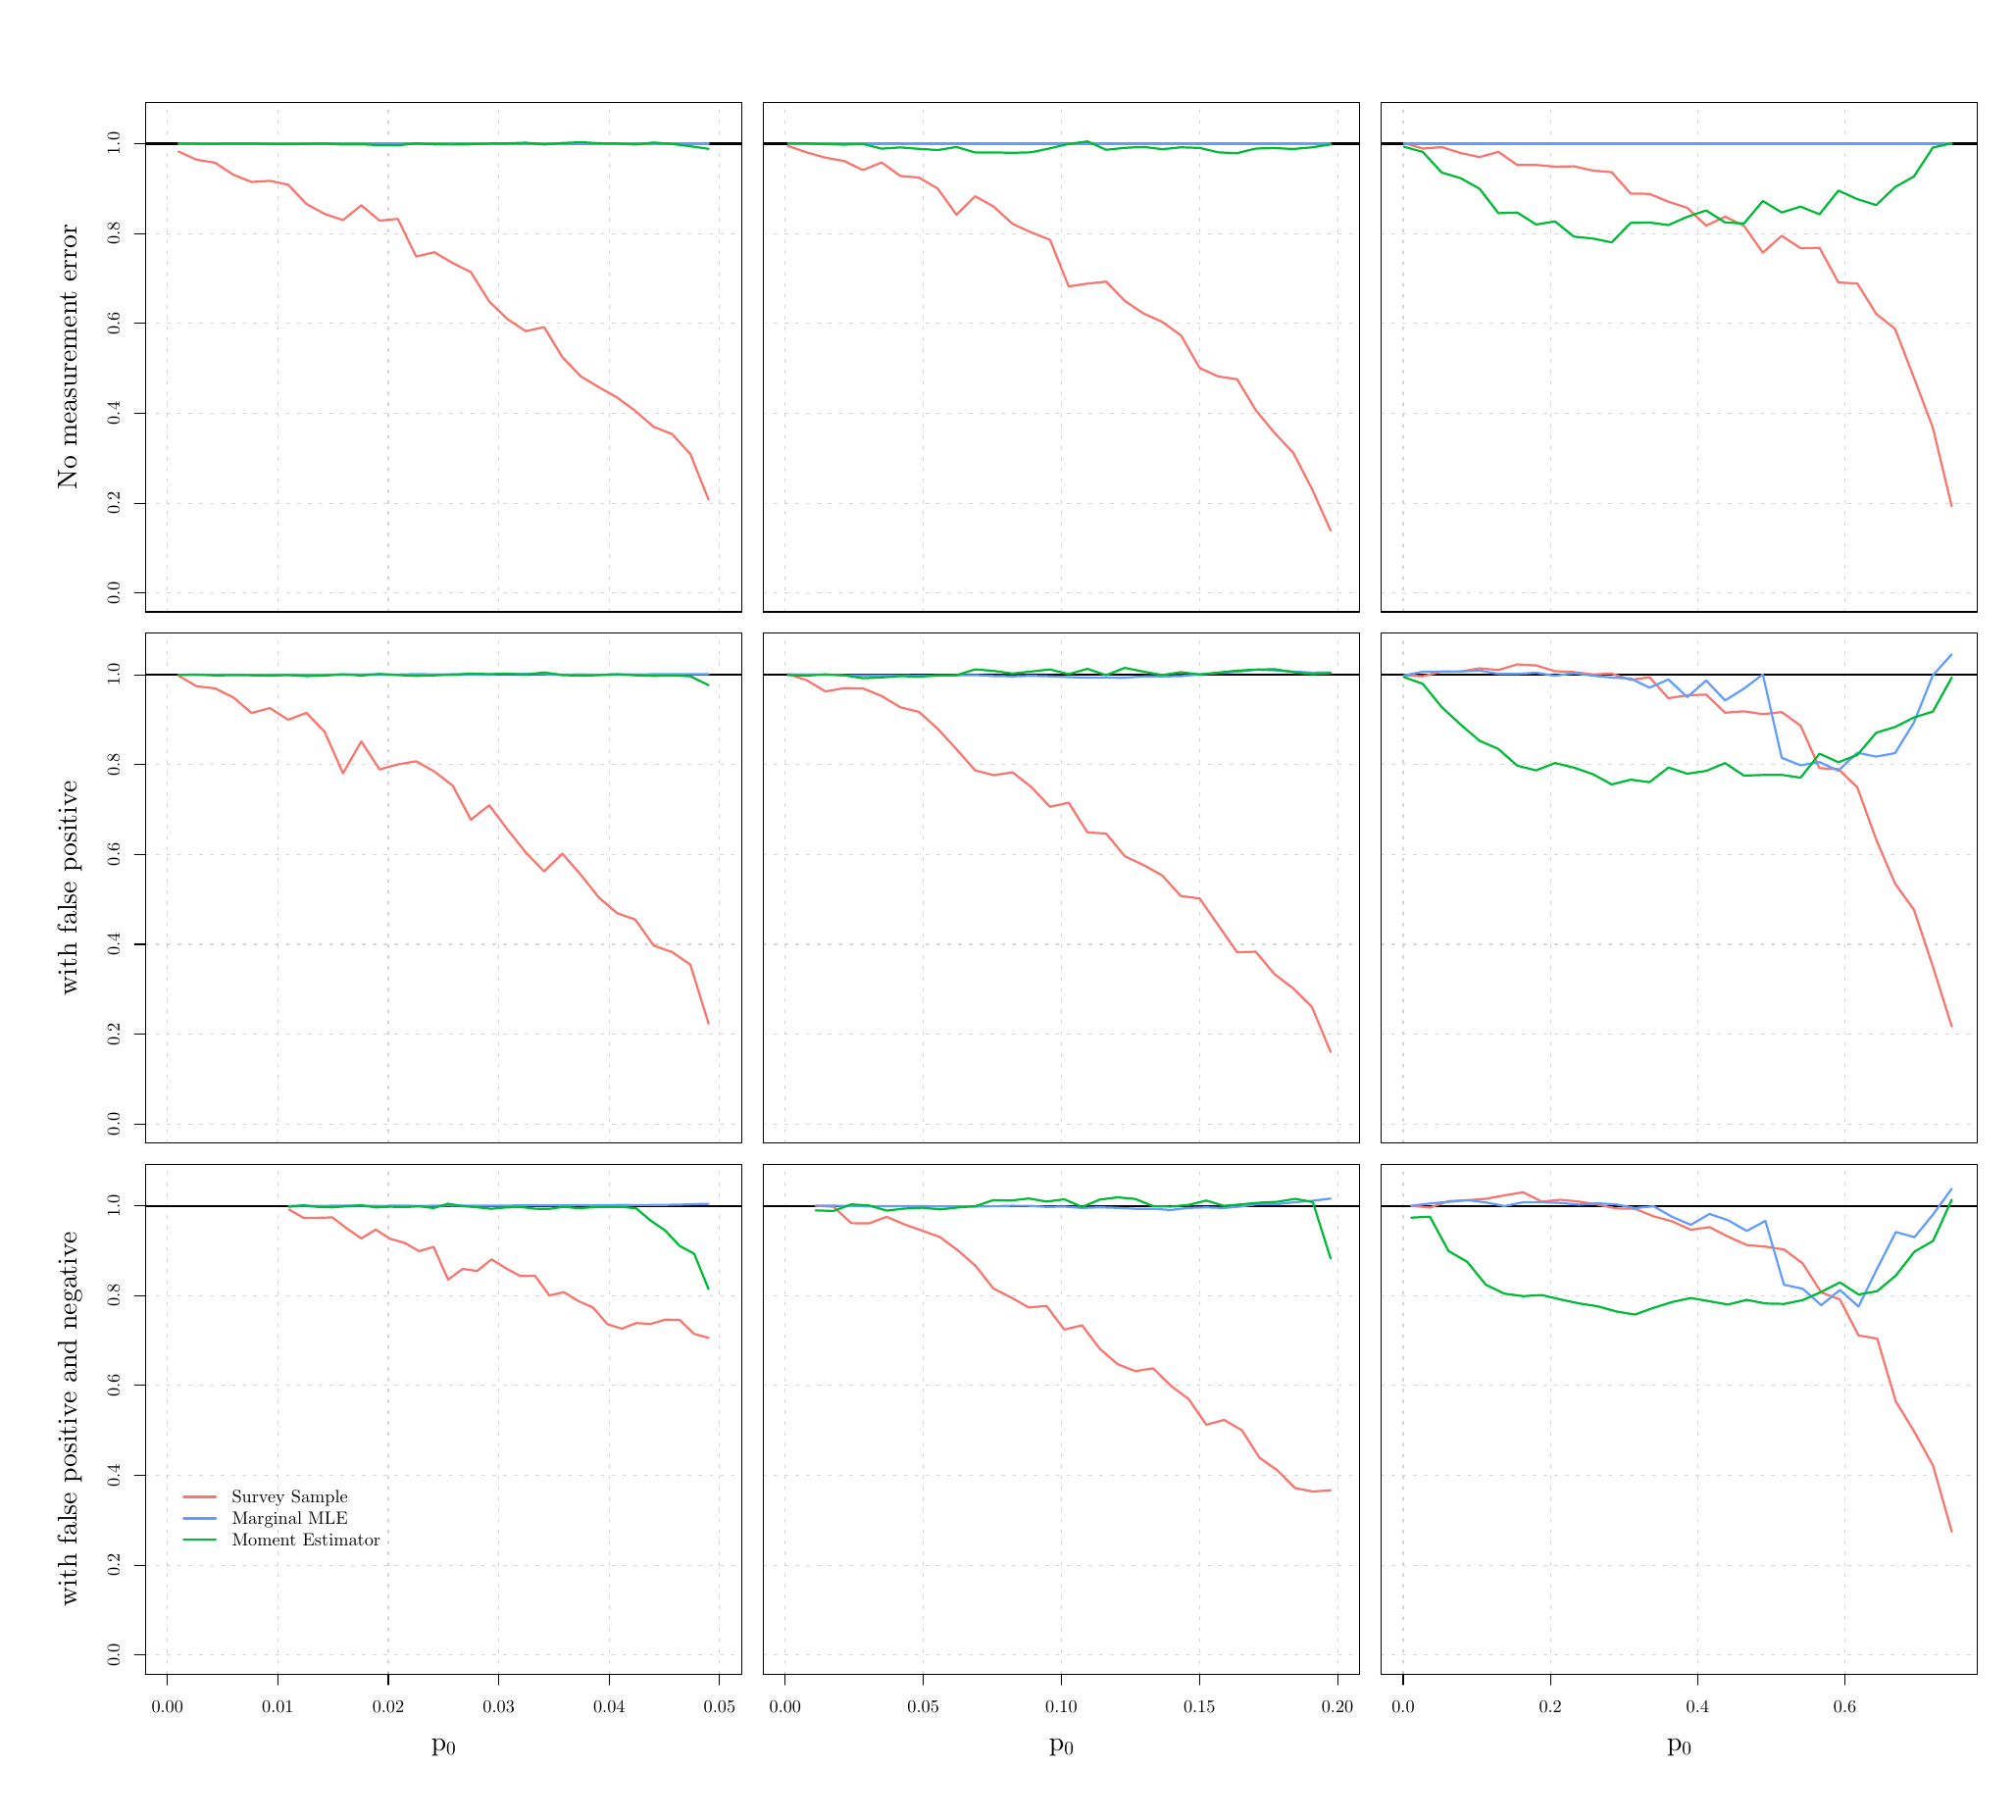
\begin{tikzpicture}[x=1pt,y=1pt]
\definecolor{fillColor}{RGB}{255,255,255}
\path[use as bounding box,fill=fillColor,fill opacity=0.00] (0,0) rectangle (722.70,650.43);
\begin{scope}
\path[clip] ( 39.60,430.98) rectangle (267.30,626.67);
\definecolor{drawColor}{RGB}{0,0,0}

\node[text=drawColor,anchor=base,inner sep=0pt, outer sep=0pt, scale=  0.66] at (153.45,404.84) {Simulation ID};

\node[text=drawColor,rotate= 90.00,anchor=base,inner sep=0pt, outer sep=0pt, scale=  0.66] at ( 18.22,528.82) {Ratio of RMSE};
\end{scope}
\begin{scope}
\path[clip] (  0.00,  0.00) rectangle (722.70,650.43);
\definecolor{drawColor}{RGB}{0,0,0}

\path[draw=drawColor,line width= 0.4pt,line join=round,line cap=round] ( 43.56,441.89) -- ( 43.56,607.48);

\path[draw=drawColor,line width= 0.4pt,line join=round,line cap=round] ( 43.56,441.89) -- ( 39.60,441.89);

\path[draw=drawColor,line width= 0.4pt,line join=round,line cap=round] ( 43.56,475.01) -- ( 39.60,475.01);

\path[draw=drawColor,line width= 0.4pt,line join=round,line cap=round] ( 43.56,508.13) -- ( 39.60,508.13);

\path[draw=drawColor,line width= 0.4pt,line join=round,line cap=round] ( 43.56,541.24) -- ( 39.60,541.24);

\path[draw=drawColor,line width= 0.4pt,line join=round,line cap=round] ( 43.56,574.36) -- ( 39.60,574.36);

\path[draw=drawColor,line width= 0.4pt,line join=round,line cap=round] ( 43.56,607.48) -- ( 39.60,607.48);

\node[text=drawColor,rotate= 90.00,anchor=base,inner sep=0pt, outer sep=0pt, scale=  0.66] at ( 34.06,441.89) {0.0};

\node[text=drawColor,rotate= 90.00,anchor=base,inner sep=0pt, outer sep=0pt, scale=  0.66] at ( 34.06,475.01) {0.2};

\node[text=drawColor,rotate= 90.00,anchor=base,inner sep=0pt, outer sep=0pt, scale=  0.66] at ( 34.06,508.13) {0.4};

\node[text=drawColor,rotate= 90.00,anchor=base,inner sep=0pt, outer sep=0pt, scale=  0.66] at ( 34.06,541.24) {0.6};

\node[text=drawColor,rotate= 90.00,anchor=base,inner sep=0pt, outer sep=0pt, scale=  0.66] at ( 34.06,574.36) {0.8};

\node[text=drawColor,rotate= 90.00,anchor=base,inner sep=0pt, outer sep=0pt, scale=  0.66] at ( 34.06,607.48) {1.0};
\end{scope}
\begin{scope}
\path[clip] ( 43.56,434.94) rectangle (263.34,622.71);
\definecolor{drawColor}{RGB}{211,211,211}

\path[draw=drawColor,line width= 0.4pt,dash pattern=on 1pt off 3pt ,line join=round,line cap=round] ( 51.70,434.94) -- ( 51.70,622.71);

\path[draw=drawColor,line width= 0.4pt,dash pattern=on 1pt off 3pt ,line join=round,line cap=round] ( 92.40,434.94) -- ( 92.40,622.71);

\path[draw=drawColor,line width= 0.4pt,dash pattern=on 1pt off 3pt ,line join=round,line cap=round] (133.10,434.94) -- (133.10,622.71);

\path[draw=drawColor,line width= 0.4pt,dash pattern=on 1pt off 3pt ,line join=round,line cap=round] (173.80,434.94) -- (173.80,622.71);

\path[draw=drawColor,line width= 0.4pt,dash pattern=on 1pt off 3pt ,line join=round,line cap=round] (214.50,434.94) -- (214.50,622.71);

\path[draw=drawColor,line width= 0.4pt,dash pattern=on 1pt off 3pt ,line join=round,line cap=round] (255.20,434.94) -- (255.20,622.71);

\path[draw=drawColor,line width= 0.4pt,dash pattern=on 1pt off 3pt ,line join=round,line cap=round] ( 43.56,441.89) -- (263.34,441.89);

\path[draw=drawColor,line width= 0.4pt,dash pattern=on 1pt off 3pt ,line join=round,line cap=round] ( 43.56,475.01) -- (263.34,475.01);

\path[draw=drawColor,line width= 0.4pt,dash pattern=on 1pt off 3pt ,line join=round,line cap=round] ( 43.56,508.13) -- (263.34,508.13);

\path[draw=drawColor,line width= 0.4pt,dash pattern=on 1pt off 3pt ,line join=round,line cap=round] ( 43.56,541.24) -- (263.34,541.24);

\path[draw=drawColor,line width= 0.4pt,dash pattern=on 1pt off 3pt ,line join=round,line cap=round] ( 43.56,574.36) -- (263.34,574.36);

\path[draw=drawColor,line width= 0.4pt,dash pattern=on 1pt off 3pt ,line join=round,line cap=round] ( 43.56,607.48) -- (263.34,607.48);
\end{scope}
\begin{scope}
\path[clip] (  0.00,  0.00) rectangle (722.70,650.43);
\definecolor{drawColor}{RGB}{0,0,0}

\path[draw=drawColor,line width= 0.4pt,line join=round,line cap=round] ( 43.56,434.94) --
	(263.34,434.94) --
	(263.34,622.71) --
	( 43.56,622.71) --
	( 43.56,434.94);
\end{scope}
\begin{scope}
\path[clip] ( 43.56,434.94) rectangle (263.34,622.71);
\definecolor{drawColor}{RGB}{0,0,0}

\path[draw=drawColor,line width= 0.8pt,line join=round,line cap=round] ( 43.56,607.48) -- (263.34,607.48);
\definecolor{drawColor}{RGB}{248,118,109}

\path[draw=drawColor,line width= 0.8pt,line join=round,line cap=round] ( 55.77,604.57) --
	( 62.51,601.55) --
	( 69.24,600.46) --
	( 75.98,596.03) --
	( 82.72,593.36) --
	( 89.45,593.78) --
	( 96.19,592.36) --
	(102.93,585.25) --
	(109.66,581.58) --
	(116.40,579.33) --
	(123.14,584.79) --
	(129.87,579.12) --
	(136.61,579.77) --
	(143.35,565.88) --
	(150.08,567.47) --
	(156.82,563.49) --
	(163.55,560.10) --
	(170.29,549.30) --
	(177.03,542.82) --
	(183.76,538.39) --
	(190.50,539.87) --
	(197.24,528.82) --
	(203.97,521.78) --
	(210.71,517.72) --
	(217.45,513.92) --
	(224.18,508.94) --
	(230.92,503.10) --
	(237.66,500.47) --
	(244.39,493.13) --
	(251.13,476.30);
\definecolor{drawColor}{RGB}{97,156,255}

\path[draw=drawColor,line width= 0.8pt,line join=round,line cap=round] ( 55.77,607.48) --
	( 62.51,607.48) --
	( 69.24,607.48) --
	( 75.98,607.48) --
	( 82.72,607.48) --
	( 89.45,607.48) --
	( 96.19,607.48) --
	(102.93,607.48) --
	(109.66,607.48) --
	(116.40,607.48) --
	(123.14,607.48) --
	(129.87,607.48) --
	(136.61,607.48) --
	(143.35,607.48) --
	(150.08,607.48) --
	(156.82,607.48) --
	(163.55,607.48) --
	(170.29,607.48) --
	(177.03,607.48) --
	(183.76,607.48) --
	(190.50,607.48) --
	(197.24,607.48) --
	(203.97,607.48) --
	(210.71,607.48) --
	(217.45,607.48) --
	(224.18,607.48) --
	(230.92,607.48) --
	(237.66,607.48) --
	(244.39,607.48) --
	(251.13,607.48);
\definecolor{drawColor}{RGB}{0,186,56}

\path[draw=drawColor,line width= 0.8pt,line join=round,line cap=round] ( 55.77,607.55) --
	( 62.51,607.45) --
	( 69.24,607.42) --
	( 75.98,607.48) --
	( 82.72,607.53) --
	( 89.45,607.34) --
	( 96.19,607.28) --
	(102.93,607.41) --
	(109.66,607.52) --
	(116.40,607.17) --
	(123.14,607.25) --
	(129.87,606.94) --
	(136.61,606.90) --
	(143.35,607.57) --
	(150.08,607.23) --
	(156.82,607.16) --
	(163.55,607.26) --
	(170.29,607.52) --
	(177.03,607.61) --
	(183.76,607.84) --
	(190.50,607.17) --
	(197.24,607.72) --
	(203.97,608.01) --
	(210.71,607.65) --
	(217.45,607.54) --
	(224.18,607.16) --
	(230.92,607.90) --
	(237.66,607.39) --
	(244.39,606.53) --
	(251.13,605.58);
\end{scope}
\begin{scope}
\path[clip] (  0.00,  0.00) rectangle (722.70,650.43);
\definecolor{drawColor}{RGB}{0,0,0}

\node[text=drawColor,rotate= 90.00,anchor=base,inner sep=0pt, outer sep=0pt, scale=  1.00] at ( 18.22,528.82) {No measurement error};
\end{scope}
\begin{scope}
\path[clip] (267.30,430.98) rectangle (495.00,626.67);
\definecolor{drawColor}{RGB}{0,0,0}

\node[text=drawColor,anchor=base,inner sep=0pt, outer sep=0pt, scale=  0.66] at (381.15,404.84) {Simulation ID};

\node[text=drawColor,rotate= 90.00,anchor=base,inner sep=0pt, outer sep=0pt, scale=  0.66] at (245.92,528.82) {Ratio of RMSE};
\end{scope}
\begin{scope}
\path[clip] (271.26,434.94) rectangle (491.04,622.71);
\definecolor{drawColor}{RGB}{211,211,211}

\path[draw=drawColor,line width= 0.4pt,dash pattern=on 1pt off 3pt ,line join=round,line cap=round] (279.40,434.94) -- (279.40,622.71);

\path[draw=drawColor,line width= 0.4pt,dash pattern=on 1pt off 3pt ,line join=round,line cap=round] (330.27,434.94) -- (330.27,622.71);

\path[draw=drawColor,line width= 0.4pt,dash pattern=on 1pt off 3pt ,line join=round,line cap=round] (381.15,434.94) -- (381.15,622.71);

\path[draw=drawColor,line width= 0.4pt,dash pattern=on 1pt off 3pt ,line join=round,line cap=round] (432.02,434.94) -- (432.02,622.71);

\path[draw=drawColor,line width= 0.4pt,dash pattern=on 1pt off 3pt ,line join=round,line cap=round] (482.90,434.94) -- (482.90,622.71);

\path[draw=drawColor,line width= 0.4pt,dash pattern=on 1pt off 3pt ,line join=round,line cap=round] (271.26,441.89) -- (491.04,441.89);

\path[draw=drawColor,line width= 0.4pt,dash pattern=on 1pt off 3pt ,line join=round,line cap=round] (271.26,475.01) -- (491.04,475.01);

\path[draw=drawColor,line width= 0.4pt,dash pattern=on 1pt off 3pt ,line join=round,line cap=round] (271.26,508.13) -- (491.04,508.13);

\path[draw=drawColor,line width= 0.4pt,dash pattern=on 1pt off 3pt ,line join=round,line cap=round] (271.26,541.24) -- (491.04,541.24);

\path[draw=drawColor,line width= 0.4pt,dash pattern=on 1pt off 3pt ,line join=round,line cap=round] (271.26,574.36) -- (491.04,574.36);

\path[draw=drawColor,line width= 0.4pt,dash pattern=on 1pt off 3pt ,line join=round,line cap=round] (271.26,607.48) -- (491.04,607.48);
\end{scope}
\begin{scope}
\path[clip] (  0.00,  0.00) rectangle (722.70,650.43);
\definecolor{drawColor}{RGB}{0,0,0}

\path[draw=drawColor,line width= 0.4pt,line join=round,line cap=round] (271.26,434.94) --
	(491.04,434.94) --
	(491.04,622.71) --
	(271.26,622.71) --
	(271.26,434.94);
\end{scope}
\begin{scope}
\path[clip] (271.26,434.94) rectangle (491.04,622.71);
\definecolor{drawColor}{RGB}{0,0,0}

\path[draw=drawColor,line width= 0.8pt,line join=round,line cap=round] (271.26,607.48) -- (491.04,607.48);
\definecolor{drawColor}{RGB}{248,118,109}

\path[draw=drawColor,line width= 0.8pt,line join=round,line cap=round] (280.42,606.63) --
	(287.31,604.26) --
	(294.21,602.32) --
	(301.10,601.09) --
	(308.00,597.74) --
	(314.89,600.56) --
	(321.78,595.59) --
	(328.68,594.98) --
	(335.57,590.93) --
	(342.47,581.31) --
	(349.36,588.09) --
	(356.26,584.25) --
	(363.15,577.91) --
	(370.05,574.79) --
	(376.94,572.06) --
	(383.83,554.87) --
	(390.73,555.91) --
	(397.62,556.64) --
	(404.52,549.52) --
	(411.41,544.91) --
	(418.31,541.78) --
	(425.20,536.85) --
	(432.10,524.82) --
	(438.99,521.69) --
	(445.88,520.67) --
	(452.78,509.28) --
	(459.67,500.91) --
	(466.57,493.60) --
	(473.46,480.30) --
	(480.36,464.91);
\definecolor{drawColor}{RGB}{97,156,255}

\path[draw=drawColor,line width= 0.8pt,line join=round,line cap=round] (280.42,607.48) --
	(287.31,607.48) --
	(294.21,607.48) --
	(301.10,607.48) --
	(308.00,607.48) --
	(314.89,607.48) --
	(321.78,607.48) --
	(328.68,607.48) --
	(335.57,607.48) --
	(342.47,607.48) --
	(349.36,607.48) --
	(356.26,607.48) --
	(363.15,607.48) --
	(370.05,607.48) --
	(376.94,607.48) --
	(383.83,607.48) --
	(390.73,607.48) --
	(397.62,607.48) --
	(404.52,607.48) --
	(411.41,607.48) --
	(418.31,607.48) --
	(425.20,607.48) --
	(432.10,607.48) --
	(438.99,607.48) --
	(445.88,607.48) --
	(452.78,607.48) --
	(459.67,607.48) --
	(466.57,607.48) --
	(473.46,607.48) --
	(480.36,607.48);
\definecolor{drawColor}{RGB}{0,186,56}

\path[draw=drawColor,line width= 0.8pt,line join=round,line cap=round] (280.42,607.63) --
	(287.31,607.56) --
	(294.21,607.32) --
	(301.10,607.13) --
	(308.00,607.36) --
	(314.89,605.64) --
	(321.78,606.10) --
	(328.68,605.57) --
	(335.57,605.13) --
	(342.47,606.26) --
	(349.36,604.22) --
	(356.26,604.24) --
	(363.15,604.13) --
	(370.05,604.30) --
	(376.94,605.76) --
	(383.83,607.38) --
	(390.73,608.31) --
	(397.62,605.23) --
	(404.52,605.94) --
	(411.41,606.28) --
	(418.31,605.45) --
	(425.20,606.13) --
	(432.10,605.91) --
	(438.99,604.28) --
	(445.88,603.97) --
	(452.78,605.69) --
	(459.67,605.85) --
	(466.57,605.53) --
	(473.46,606.12) --
	(480.36,607.20);
\end{scope}
\begin{scope}
\path[clip] (495.00,430.98) rectangle (722.70,626.67);
\definecolor{drawColor}{RGB}{0,0,0}

\node[text=drawColor,anchor=base,inner sep=0pt, outer sep=0pt, scale=  0.66] at (608.85,404.84) {Simulation ID};

\node[text=drawColor,rotate= 90.00,anchor=base,inner sep=0pt, outer sep=0pt, scale=  0.66] at (473.62,528.82) {Ratio of RMSE};
\end{scope}
\begin{scope}
\path[clip] (498.96,434.94) rectangle (718.74,622.71);
\definecolor{drawColor}{RGB}{211,211,211}

\path[draw=drawColor,line width= 0.4pt,dash pattern=on 1pt off 3pt ,line join=round,line cap=round] (507.10,434.94) -- (507.10,622.71);

\path[draw=drawColor,line width= 0.4pt,dash pattern=on 1pt off 3pt ,line join=round,line cap=round] (561.37,434.94) -- (561.37,622.71);

\path[draw=drawColor,line width= 0.4pt,dash pattern=on 1pt off 3pt ,line join=round,line cap=round] (615.63,434.94) -- (615.63,622.71);

\path[draw=drawColor,line width= 0.4pt,dash pattern=on 1pt off 3pt ,line join=round,line cap=round] (669.90,434.94) -- (669.90,622.71);

\path[draw=drawColor,line width= 0.4pt,dash pattern=on 1pt off 3pt ,line join=round,line cap=round] (498.96,441.89) -- (718.74,441.89);

\path[draw=drawColor,line width= 0.4pt,dash pattern=on 1pt off 3pt ,line join=round,line cap=round] (498.96,475.01) -- (718.74,475.01);

\path[draw=drawColor,line width= 0.4pt,dash pattern=on 1pt off 3pt ,line join=round,line cap=round] (498.96,508.13) -- (718.74,508.13);

\path[draw=drawColor,line width= 0.4pt,dash pattern=on 1pt off 3pt ,line join=round,line cap=round] (498.96,541.24) -- (718.74,541.24);

\path[draw=drawColor,line width= 0.4pt,dash pattern=on 1pt off 3pt ,line join=round,line cap=round] (498.96,574.36) -- (718.74,574.36);

\path[draw=drawColor,line width= 0.4pt,dash pattern=on 1pt off 3pt ,line join=round,line cap=round] (498.96,607.48) -- (718.74,607.48);
\end{scope}
\begin{scope}
\path[clip] (  0.00,  0.00) rectangle (722.70,650.43);
\definecolor{drawColor}{RGB}{0,0,0}

\path[draw=drawColor,line width= 0.4pt,line join=round,line cap=round] (498.96,434.94) --
	(718.74,434.94) --
	(718.74,622.71) --
	(498.96,622.71) --
	(498.96,434.94);
\end{scope}
\begin{scope}
\path[clip] (498.96,434.94) rectangle (718.74,622.71);
\definecolor{drawColor}{RGB}{0,0,0}

\path[draw=drawColor,line width= 0.8pt,line join=round,line cap=round] (498.96,607.48) -- (718.74,607.48);
\definecolor{drawColor}{RGB}{248,118,109}

\path[draw=drawColor,line width= 0.8pt,line join=round,line cap=round] (507.37,607.76) --
	(514.33,605.66) --
	(521.29,606.20) --
	(528.25,604.05) --
	(535.22,602.54) --
	(542.18,604.46) --
	(549.14,599.61) --
	(556.10,599.63) --
	(563.06,599.01) --
	(570.02,599.14) --
	(576.98,597.57) --
	(583.94,596.97) --
	(590.90,589.10) --
	(597.87,588.98) --
	(604.83,586.09) --
	(611.79,583.83) --
	(618.75,577.25) --
	(625.71,580.57) --
	(632.67,577.21) --
	(639.63,567.33) --
	(646.59,573.54) --
	(653.55,568.94) --
	(660.52,569.11) --
	(667.48,556.34) --
	(674.44,555.95) --
	(681.40,544.78) --
	(688.36,539.23) --
	(695.32,521.21) --
	(702.28,502.85) --
	(709.24,473.88);
\definecolor{drawColor}{RGB}{97,156,255}

\path[draw=drawColor,line width= 0.8pt,line join=round,line cap=round] (507.37,607.48) --
	(514.33,607.48) --
	(521.29,607.48) --
	(528.25,607.48) --
	(535.22,607.48) --
	(542.18,607.48) --
	(549.14,607.48) --
	(556.10,607.48) --
	(563.06,607.48) --
	(570.02,607.48) --
	(576.98,607.48) --
	(583.94,607.48) --
	(590.90,607.48) --
	(597.87,607.48) --
	(604.83,607.48) --
	(611.79,607.48) --
	(618.75,607.48) --
	(625.71,607.48) --
	(632.67,607.48) --
	(639.63,607.48) --
	(646.59,607.48) --
	(653.55,607.48) --
	(660.52,607.48) --
	(667.48,607.48) --
	(674.44,607.48) --
	(681.40,607.48) --
	(688.36,607.48) --
	(695.32,607.48) --
	(702.28,607.48) --
	(709.24,607.48);
\definecolor{drawColor}{RGB}{0,186,56}

\path[draw=drawColor,line width= 0.8pt,line join=round,line cap=round] (507.37,606.35) --
	(514.33,604.43) --
	(521.29,596.84) --
	(528.25,594.77) --
	(535.22,590.89) --
	(542.18,581.86) --
	(549.14,582.09) --
	(556.10,577.70) --
	(563.06,578.82) --
	(570.02,573.22) --
	(576.98,572.53) --
	(583.94,571.11) --
	(590.90,578.26) --
	(597.87,578.42) --
	(604.83,577.49) --
	(611.79,580.53) --
	(618.75,582.87) --
	(625.71,578.47) --
	(632.67,578.07) --
	(639.63,586.34) --
	(646.59,582.14) --
	(653.55,584.29) --
	(660.52,581.47) --
	(667.48,590.19) --
	(674.44,587.05) --
	(681.40,584.85) --
	(688.36,591.47) --
	(695.32,595.39) --
	(702.28,606.04) --
	(709.24,607.61);
\end{scope}
\begin{scope}
\path[clip] ( 39.60,235.29) rectangle (267.30,430.98);
\definecolor{drawColor}{RGB}{0,0,0}

\node[text=drawColor,anchor=base,inner sep=0pt, outer sep=0pt, scale=  0.66] at (153.45,209.15) {Simulation ID};

\node[text=drawColor,rotate= 90.00,anchor=base,inner sep=0pt, outer sep=0pt, scale=  0.66] at ( 18.22,333.13) {Ratio of RMSE};
\end{scope}
\begin{scope}
\path[clip] (  0.00,  0.00) rectangle (722.70,650.43);
\definecolor{drawColor}{RGB}{0,0,0}

\path[draw=drawColor,line width= 0.4pt,line join=round,line cap=round] ( 43.56,246.20) -- ( 43.56,411.79);

\path[draw=drawColor,line width= 0.4pt,line join=round,line cap=round] ( 43.56,246.20) -- ( 39.60,246.20);

\path[draw=drawColor,line width= 0.4pt,line join=round,line cap=round] ( 43.56,279.32) -- ( 39.60,279.32);

\path[draw=drawColor,line width= 0.4pt,line join=round,line cap=round] ( 43.56,312.44) -- ( 39.60,312.44);

\path[draw=drawColor,line width= 0.4pt,line join=round,line cap=round] ( 43.56,345.55) -- ( 39.60,345.55);

\path[draw=drawColor,line width= 0.4pt,line join=round,line cap=round] ( 43.56,378.67) -- ( 39.60,378.67);

\path[draw=drawColor,line width= 0.4pt,line join=round,line cap=round] ( 43.56,411.79) -- ( 39.60,411.79);

\node[text=drawColor,rotate= 90.00,anchor=base,inner sep=0pt, outer sep=0pt, scale=  0.66] at ( 34.06,246.20) {0.0};

\node[text=drawColor,rotate= 90.00,anchor=base,inner sep=0pt, outer sep=0pt, scale=  0.66] at ( 34.06,279.32) {0.2};

\node[text=drawColor,rotate= 90.00,anchor=base,inner sep=0pt, outer sep=0pt, scale=  0.66] at ( 34.06,312.44) {0.4};

\node[text=drawColor,rotate= 90.00,anchor=base,inner sep=0pt, outer sep=0pt, scale=  0.66] at ( 34.06,345.55) {0.6};

\node[text=drawColor,rotate= 90.00,anchor=base,inner sep=0pt, outer sep=0pt, scale=  0.66] at ( 34.06,378.67) {0.8};

\node[text=drawColor,rotate= 90.00,anchor=base,inner sep=0pt, outer sep=0pt, scale=  0.66] at ( 34.06,411.79) {1.0};
\end{scope}
\begin{scope}
\path[clip] ( 43.56,239.25) rectangle (263.34,427.02);
\definecolor{drawColor}{RGB}{211,211,211}

\path[draw=drawColor,line width= 0.4pt,dash pattern=on 1pt off 3pt ,line join=round,line cap=round] ( 51.70,239.25) -- ( 51.70,427.02);

\path[draw=drawColor,line width= 0.4pt,dash pattern=on 1pt off 3pt ,line join=round,line cap=round] ( 92.40,239.25) -- ( 92.40,427.02);

\path[draw=drawColor,line width= 0.4pt,dash pattern=on 1pt off 3pt ,line join=round,line cap=round] (133.10,239.25) -- (133.10,427.02);

\path[draw=drawColor,line width= 0.4pt,dash pattern=on 1pt off 3pt ,line join=round,line cap=round] (173.80,239.25) -- (173.80,427.02);

\path[draw=drawColor,line width= 0.4pt,dash pattern=on 1pt off 3pt ,line join=round,line cap=round] (214.50,239.25) -- (214.50,427.02);

\path[draw=drawColor,line width= 0.4pt,dash pattern=on 1pt off 3pt ,line join=round,line cap=round] (255.20,239.25) -- (255.20,427.02);

\path[draw=drawColor,line width= 0.4pt,dash pattern=on 1pt off 3pt ,line join=round,line cap=round] ( 43.56,246.20) -- (263.34,246.20);

\path[draw=drawColor,line width= 0.4pt,dash pattern=on 1pt off 3pt ,line join=round,line cap=round] ( 43.56,279.32) -- (263.34,279.32);

\path[draw=drawColor,line width= 0.4pt,dash pattern=on 1pt off 3pt ,line join=round,line cap=round] ( 43.56,312.44) -- (263.34,312.44);

\path[draw=drawColor,line width= 0.4pt,dash pattern=on 1pt off 3pt ,line join=round,line cap=round] ( 43.56,345.55) -- (263.34,345.55);

\path[draw=drawColor,line width= 0.4pt,dash pattern=on 1pt off 3pt ,line join=round,line cap=round] ( 43.56,378.67) -- (263.34,378.67);

\path[draw=drawColor,line width= 0.4pt,dash pattern=on 1pt off 3pt ,line join=round,line cap=round] ( 43.56,411.79) -- (263.34,411.79);
\end{scope}
\begin{scope}
\path[clip] (  0.00,  0.00) rectangle (722.70,650.43);
\definecolor{drawColor}{RGB}{0,0,0}

\path[draw=drawColor,line width= 0.4pt,line join=round,line cap=round] ( 43.56,239.25) --
	(263.34,239.25) --
	(263.34,427.02) --
	( 43.56,427.02) --
	( 43.56,239.25);
\end{scope}
\begin{scope}
\path[clip] ( 43.56,239.25) rectangle (263.34,427.02);
\definecolor{drawColor}{RGB}{0,0,0}

\path[draw=drawColor,line width= 0.8pt,line join=round,line cap=round] ( 43.56,411.79) -- (263.34,411.79);
\definecolor{drawColor}{RGB}{248,118,109}

\path[draw=drawColor,line width= 0.8pt,line join=round,line cap=round] ( 55.77,411.43) --
	( 62.51,407.51) --
	( 69.24,406.77) --
	( 75.98,403.43) --
	( 82.72,397.69) --
	( 89.45,399.50) --
	( 96.19,395.20) --
	(102.93,397.74) --
	(109.66,390.71) --
	(116.40,375.47) --
	(123.14,387.22) --
	(129.87,376.89) --
	(136.61,378.75) --
	(143.35,379.89) --
	(150.08,376.12) --
	(156.82,370.93) --
	(163.55,358.38) --
	(170.29,363.69) --
	(177.03,354.74) --
	(183.76,346.27) --
	(190.50,339.33) --
	(197.24,345.85) --
	(203.97,338.15) --
	(210.71,329.66) --
	(217.45,323.92) --
	(224.18,321.52) --
	(230.92,311.96) --
	(237.66,309.60) --
	(244.39,304.96) --
	(251.13,283.19);
\definecolor{drawColor}{RGB}{97,156,255}

\path[draw=drawColor,line width= 0.8pt,line join=round,line cap=round] ( 55.77,411.76) --
	( 62.51,411.84) --
	( 69.24,411.77) --
	( 75.98,411.81) --
	( 82.72,411.76) --
	( 89.45,411.78) --
	( 96.19,411.80) --
	(102.93,411.80) --
	(109.66,411.82) --
	(116.40,411.84) --
	(123.14,411.92) --
	(129.87,411.87) --
	(136.61,411.85) --
	(143.35,412.02) --
	(150.08,411.91) --
	(156.82,411.96) --
	(163.55,411.93) --
	(170.29,411.93) --
	(177.03,411.97) --
	(183.76,412.06) --
	(190.50,411.96) --
	(197.24,411.83) --
	(203.97,411.89) --
	(210.71,411.82) --
	(217.45,411.91) --
	(224.18,411.92) --
	(230.92,411.97) --
	(237.66,411.99) --
	(244.39,411.98) --
	(251.13,412.02);
\definecolor{drawColor}{RGB}{0,186,56}

\path[draw=drawColor,line width= 0.8pt,line join=round,line cap=round] ( 55.77,411.72) --
	( 62.51,411.81) --
	( 69.24,411.54) --
	( 75.98,411.62) --
	( 82.72,411.58) --
	( 89.45,411.45) --
	( 96.19,411.66) --
	(102.93,411.29) --
	(109.66,411.46) --
	(116.40,411.97) --
	(123.14,411.48) --
	(129.87,412.07) --
	(136.61,411.68) --
	(143.35,411.36) --
	(150.08,411.57) --
	(156.82,411.81) --
	(163.55,412.18) --
	(170.29,412.00) --
	(177.03,412.19) --
	(183.76,411.87) --
	(190.50,412.63) --
	(197.24,411.67) --
	(203.97,411.44) --
	(210.71,411.63) --
	(217.45,411.98) --
	(224.18,411.57) --
	(230.92,411.37) --
	(237.66,411.51) --
	(244.39,411.24) --
	(251.13,407.92);
\end{scope}
\begin{scope}
\path[clip] (  0.00,  0.00) rectangle (722.70,650.43);
\definecolor{drawColor}{RGB}{0,0,0}

\node[text=drawColor,rotate= 90.00,anchor=base,inner sep=0pt, outer sep=0pt, scale=  1.00] at ( 18.22,333.13) {with false positive};
\end{scope}
\begin{scope}
\path[clip] (267.30,235.29) rectangle (495.00,430.98);
\definecolor{drawColor}{RGB}{0,0,0}

\node[text=drawColor,anchor=base,inner sep=0pt, outer sep=0pt, scale=  0.66] at (381.15,209.15) {Simulation ID};

\node[text=drawColor,rotate= 90.00,anchor=base,inner sep=0pt, outer sep=0pt, scale=  0.66] at (245.92,333.13) {Ratio of RMSE};
\end{scope}
\begin{scope}
\path[clip] (271.26,239.25) rectangle (491.04,427.02);
\definecolor{drawColor}{RGB}{211,211,211}

\path[draw=drawColor,line width= 0.4pt,dash pattern=on 1pt off 3pt ,line join=round,line cap=round] (279.40,239.25) -- (279.40,427.02);

\path[draw=drawColor,line width= 0.4pt,dash pattern=on 1pt off 3pt ,line join=round,line cap=round] (330.27,239.25) -- (330.27,427.02);

\path[draw=drawColor,line width= 0.4pt,dash pattern=on 1pt off 3pt ,line join=round,line cap=round] (381.15,239.25) -- (381.15,427.02);

\path[draw=drawColor,line width= 0.4pt,dash pattern=on 1pt off 3pt ,line join=round,line cap=round] (432.02,239.25) -- (432.02,427.02);

\path[draw=drawColor,line width= 0.4pt,dash pattern=on 1pt off 3pt ,line join=round,line cap=round] (482.90,239.25) -- (482.90,427.02);

\path[draw=drawColor,line width= 0.4pt,dash pattern=on 1pt off 3pt ,line join=round,line cap=round] (271.26,246.20) -- (491.04,246.20);

\path[draw=drawColor,line width= 0.4pt,dash pattern=on 1pt off 3pt ,line join=round,line cap=round] (271.26,279.32) -- (491.04,279.32);

\path[draw=drawColor,line width= 0.4pt,dash pattern=on 1pt off 3pt ,line join=round,line cap=round] (271.26,312.44) -- (491.04,312.44);

\path[draw=drawColor,line width= 0.4pt,dash pattern=on 1pt off 3pt ,line join=round,line cap=round] (271.26,345.55) -- (491.04,345.55);

\path[draw=drawColor,line width= 0.4pt,dash pattern=on 1pt off 3pt ,line join=round,line cap=round] (271.26,378.67) -- (491.04,378.67);

\path[draw=drawColor,line width= 0.4pt,dash pattern=on 1pt off 3pt ,line join=round,line cap=round] (271.26,411.79) -- (491.04,411.79);
\end{scope}
\begin{scope}
\path[clip] (  0.00,  0.00) rectangle (722.70,650.43);
\definecolor{drawColor}{RGB}{0,0,0}

\path[draw=drawColor,line width= 0.4pt,line join=round,line cap=round] (271.26,239.25) --
	(491.04,239.25) --
	(491.04,427.02) --
	(271.26,427.02) --
	(271.26,239.25);
\end{scope}
\begin{scope}
\path[clip] (271.26,239.25) rectangle (491.04,427.02);
\definecolor{drawColor}{RGB}{0,0,0}

\path[draw=drawColor,line width= 0.8pt,line join=round,line cap=round] (271.26,411.79) -- (491.04,411.79);
\definecolor{drawColor}{RGB}{248,118,109}

\path[draw=drawColor,line width= 0.8pt,line join=round,line cap=round] (280.42,412.03) --
	(287.31,409.74) --
	(294.21,405.63) --
	(301.10,406.85) --
	(308.00,406.76) --
	(314.89,403.95) --
	(321.78,399.79) --
	(328.68,398.09) --
	(335.57,391.86) --
	(342.47,384.34) --
	(349.36,376.54) --
	(356.26,374.77) --
	(363.15,375.83) --
	(370.05,370.39) --
	(376.94,363.13) --
	(383.83,364.63) --
	(390.73,353.68) --
	(397.62,353.28) --
	(404.52,344.88) --
	(411.41,341.67) --
	(418.31,337.79) --
	(425.20,330.22) --
	(432.10,329.35) --
	(438.99,319.41) --
	(445.88,309.54) --
	(452.78,309.72) --
	(459.67,301.44) --
	(466.57,296.20) --
	(473.46,289.38) --
	(480.36,272.76);
\definecolor{drawColor}{RGB}{97,156,255}

\path[draw=drawColor,line width= 0.8pt,line join=round,line cap=round] (280.42,411.88) --
	(287.31,411.88) --
	(294.21,411.85) --
	(301.10,411.54) --
	(308.00,411.56) --
	(314.89,411.52) --
	(321.78,411.58) --
	(328.68,411.43) --
	(335.57,411.53) --
	(342.47,411.57) --
	(349.36,411.67) --
	(356.26,411.31) --
	(363.15,411.19) --
	(370.05,411.38) --
	(376.94,411.21) --
	(383.83,410.90) --
	(390.73,410.69) --
	(397.62,410.69) --
	(404.52,410.67) --
	(411.41,411.16) --
	(418.31,411.16) --
	(425.20,411.28) --
	(432.10,411.88) --
	(438.99,412.44) --
	(445.88,412.86) --
	(452.78,413.64) --
	(459.67,413.39) --
	(466.57,412.95) --
	(473.46,412.57) --
	(480.36,412.66);
\definecolor{drawColor}{RGB}{0,186,56}

\path[draw=drawColor,line width= 0.8pt,line join=round,line cap=round] (280.42,411.65) --
	(287.31,411.47) --
	(294.21,411.91) --
	(301.10,411.59) --
	(308.00,410.50) --
	(314.89,410.78) --
	(321.78,411.29) --
	(328.68,411.10) --
	(335.57,411.49) --
	(342.47,411.63) --
	(349.36,413.75) --
	(356.26,413.19) --
	(363.15,412.22) --
	(370.05,412.98) --
	(376.94,413.73) --
	(383.83,412.00) --
	(390.73,413.96) --
	(397.62,411.62) --
	(404.52,414.32) --
	(411.41,412.92) --
	(418.31,411.67) --
	(425.20,412.73) --
	(432.10,411.88) --
	(438.99,412.58) --
	(445.88,413.30) --
	(452.78,413.66) --
	(459.67,413.84) --
	(466.57,412.73) --
	(473.46,411.97) --
	(480.36,412.37);
\end{scope}
\begin{scope}
\path[clip] (495.00,235.29) rectangle (722.70,430.98);
\definecolor{drawColor}{RGB}{0,0,0}

\node[text=drawColor,anchor=base,inner sep=0pt, outer sep=0pt, scale=  0.66] at (608.85,209.15) {Simulation ID};

\node[text=drawColor,rotate= 90.00,anchor=base,inner sep=0pt, outer sep=0pt, scale=  0.66] at (473.62,333.13) {Ratio of RMSE};
\end{scope}
\begin{scope}
\path[clip] (498.96,239.25) rectangle (718.74,427.02);
\definecolor{drawColor}{RGB}{211,211,211}

\path[draw=drawColor,line width= 0.4pt,dash pattern=on 1pt off 3pt ,line join=round,line cap=round] (507.10,239.25) -- (507.10,427.02);

\path[draw=drawColor,line width= 0.4pt,dash pattern=on 1pt off 3pt ,line join=round,line cap=round] (561.37,239.25) -- (561.37,427.02);

\path[draw=drawColor,line width= 0.4pt,dash pattern=on 1pt off 3pt ,line join=round,line cap=round] (615.63,239.25) -- (615.63,427.02);

\path[draw=drawColor,line width= 0.4pt,dash pattern=on 1pt off 3pt ,line join=round,line cap=round] (669.90,239.25) -- (669.90,427.02);

\path[draw=drawColor,line width= 0.4pt,dash pattern=on 1pt off 3pt ,line join=round,line cap=round] (498.96,246.20) -- (718.74,246.20);

\path[draw=drawColor,line width= 0.4pt,dash pattern=on 1pt off 3pt ,line join=round,line cap=round] (498.96,279.32) -- (718.74,279.32);

\path[draw=drawColor,line width= 0.4pt,dash pattern=on 1pt off 3pt ,line join=round,line cap=round] (498.96,312.44) -- (718.74,312.44);

\path[draw=drawColor,line width= 0.4pt,dash pattern=on 1pt off 3pt ,line join=round,line cap=round] (498.96,345.55) -- (718.74,345.55);

\path[draw=drawColor,line width= 0.4pt,dash pattern=on 1pt off 3pt ,line join=round,line cap=round] (498.96,378.67) -- (718.74,378.67);

\path[draw=drawColor,line width= 0.4pt,dash pattern=on 1pt off 3pt ,line join=round,line cap=round] (498.96,411.79) -- (718.74,411.79);
\end{scope}
\begin{scope}
\path[clip] (  0.00,  0.00) rectangle (722.70,650.43);
\definecolor{drawColor}{RGB}{0,0,0}

\path[draw=drawColor,line width= 0.4pt,line join=round,line cap=round] (498.96,239.25) --
	(718.74,239.25) --
	(718.74,427.02) --
	(498.96,427.02) --
	(498.96,239.25);
\end{scope}
\begin{scope}
\path[clip] (498.96,239.25) rectangle (718.74,427.02);
\definecolor{drawColor}{RGB}{0,0,0}

\path[draw=drawColor,line width= 0.8pt,line join=round,line cap=round] (498.96,411.79) -- (718.74,411.79);
\definecolor{drawColor}{RGB}{248,118,109}

\path[draw=drawColor,line width= 0.8pt,line join=round,line cap=round] (507.37,411.59) --
	(514.33,411.21) --
	(521.29,412.96) --
	(528.25,412.94) --
	(535.22,414.16) --
	(542.18,413.51) --
	(549.14,415.60) --
	(556.10,415.21) --
	(563.06,413.09) --
	(570.02,412.76) --
	(576.98,411.90) --
	(583.94,412.19) --
	(590.90,409.88) --
	(597.87,410.86) --
	(604.83,403.14) --
	(611.79,404.22) --
	(618.75,404.47) --
	(625.71,397.81) --
	(632.67,398.32) --
	(639.63,397.26) --
	(646.59,398.02) --
	(653.55,393.00) --
	(660.52,377.36) --
	(667.48,376.99) --
	(674.44,370.30) --
	(681.40,351.09) --
	(688.36,334.82) --
	(695.32,325.19) --
	(702.28,304.33) --
	(709.24,282.22);
\definecolor{drawColor}{RGB}{97,156,255}

\path[draw=drawColor,line width= 0.8pt,line join=round,line cap=round] (507.37,411.51) --
	(514.33,412.91) --
	(521.29,412.88) --
	(528.25,412.98) --
	(535.22,413.33) --
	(542.18,412.11) --
	(549.14,412.07) --
	(556.10,412.53) --
	(563.06,411.40) --
	(570.02,412.36) --
	(576.98,411.43) --
	(583.94,410.74) --
	(590.90,410.39) --
	(597.87,407.01) --
	(604.83,410.04) --
	(611.79,403.53) --
	(618.75,409.66) --
	(625.71,402.31) --
	(632.67,406.66) --
	(639.63,411.92) --
	(646.59,381.19) --
	(653.55,378.42) --
	(660.52,379.56) --
	(667.48,376.43) --
	(674.44,383.06) --
	(681.40,381.60) --
	(688.36,382.90) --
	(695.32,394.20) --
	(702.28,411.57) --
	(709.24,419.31);
\definecolor{drawColor}{RGB}{0,186,56}

\path[draw=drawColor,line width= 0.8pt,line join=round,line cap=round] (507.37,410.91) --
	(514.33,408.42) --
	(521.29,399.87) --
	(528.25,393.43) --
	(535.22,387.46) --
	(542.18,384.43) --
	(549.14,378.28) --
	(556.10,376.54) --
	(563.06,379.24) --
	(570.02,377.55) --
	(576.98,375.16) --
	(583.94,371.35) --
	(590.90,373.12) --
	(597.87,372.19) --
	(604.83,377.58) --
	(611.79,375.32) --
	(618.75,376.34) --
	(625.71,379.22) --
	(632.67,374.63) --
	(639.63,374.84) --
	(646.59,374.89) --
	(653.55,373.84) --
	(660.52,382.69) --
	(667.48,379.54) --
	(674.44,382.21) --
	(681.40,390.41) --
	(688.36,392.54) --
	(695.32,396.04) --
	(702.28,398.20) --
	(709.24,410.74);
\end{scope}
\begin{scope}
\path[clip] ( 39.60, 39.60) rectangle (267.30,235.29);
\definecolor{drawColor}{RGB}{0,0,0}

\node[text=drawColor,anchor=base,inner sep=0pt, outer sep=0pt, scale=  0.66] at (153.45, 13.46) {Simulation ID};

\node[text=drawColor,rotate= 90.00,anchor=base,inner sep=0pt, outer sep=0pt, scale=  0.66] at ( 18.22,137.45) {Ratio of RMSE};
\end{scope}
\begin{scope}
\path[clip] (  0.00,  0.00) rectangle (722.70,650.43);
\definecolor{drawColor}{RGB}{0,0,0}

\path[draw=drawColor,line width= 0.4pt,line join=round,line cap=round] ( 43.56, 50.51) -- ( 43.56,216.10);

\path[draw=drawColor,line width= 0.4pt,line join=round,line cap=round] ( 43.56, 50.51) -- ( 39.60, 50.51);

\path[draw=drawColor,line width= 0.4pt,line join=round,line cap=round] ( 43.56, 83.63) -- ( 39.60, 83.63);

\path[draw=drawColor,line width= 0.4pt,line join=round,line cap=round] ( 43.56,116.75) -- ( 39.60,116.75);

\path[draw=drawColor,line width= 0.4pt,line join=round,line cap=round] ( 43.56,149.86) -- ( 39.60,149.86);

\path[draw=drawColor,line width= 0.4pt,line join=round,line cap=round] ( 43.56,182.98) -- ( 39.60,182.98);

\path[draw=drawColor,line width= 0.4pt,line join=round,line cap=round] ( 43.56,216.10) -- ( 39.60,216.10);

\node[text=drawColor,rotate= 90.00,anchor=base,inner sep=0pt, outer sep=0pt, scale=  0.66] at ( 34.06, 50.51) {0.0};

\node[text=drawColor,rotate= 90.00,anchor=base,inner sep=0pt, outer sep=0pt, scale=  0.66] at ( 34.06, 83.63) {0.2};

\node[text=drawColor,rotate= 90.00,anchor=base,inner sep=0pt, outer sep=0pt, scale=  0.66] at ( 34.06,116.75) {0.4};

\node[text=drawColor,rotate= 90.00,anchor=base,inner sep=0pt, outer sep=0pt, scale=  0.66] at ( 34.06,149.86) {0.6};

\node[text=drawColor,rotate= 90.00,anchor=base,inner sep=0pt, outer sep=0pt, scale=  0.66] at ( 34.06,182.98) {0.8};

\node[text=drawColor,rotate= 90.00,anchor=base,inner sep=0pt, outer sep=0pt, scale=  0.66] at ( 34.06,216.10) {1.0};
\end{scope}
\begin{scope}
\path[clip] ( 43.56, 43.56) rectangle (263.34,231.33);
\definecolor{drawColor}{RGB}{211,211,211}

\path[draw=drawColor,line width= 0.4pt,dash pattern=on 1pt off 3pt ,line join=round,line cap=round] ( 51.70, 43.56) -- ( 51.70,231.33);

\path[draw=drawColor,line width= 0.4pt,dash pattern=on 1pt off 3pt ,line join=round,line cap=round] ( 92.40, 43.56) -- ( 92.40,231.33);

\path[draw=drawColor,line width= 0.4pt,dash pattern=on 1pt off 3pt ,line join=round,line cap=round] (133.10, 43.56) -- (133.10,231.33);

\path[draw=drawColor,line width= 0.4pt,dash pattern=on 1pt off 3pt ,line join=round,line cap=round] (173.80, 43.56) -- (173.80,231.33);

\path[draw=drawColor,line width= 0.4pt,dash pattern=on 1pt off 3pt ,line join=round,line cap=round] (214.50, 43.56) -- (214.50,231.33);

\path[draw=drawColor,line width= 0.4pt,dash pattern=on 1pt off 3pt ,line join=round,line cap=round] (255.20, 43.56) -- (255.20,231.33);

\path[draw=drawColor,line width= 0.4pt,dash pattern=on 1pt off 3pt ,line join=round,line cap=round] ( 43.56, 50.51) -- (263.34, 50.51);

\path[draw=drawColor,line width= 0.4pt,dash pattern=on 1pt off 3pt ,line join=round,line cap=round] ( 43.56, 83.63) -- (263.34, 83.63);

\path[draw=drawColor,line width= 0.4pt,dash pattern=on 1pt off 3pt ,line join=round,line cap=round] ( 43.56,116.75) -- (263.34,116.75);

\path[draw=drawColor,line width= 0.4pt,dash pattern=on 1pt off 3pt ,line join=round,line cap=round] ( 43.56,149.86) -- (263.34,149.86);

\path[draw=drawColor,line width= 0.4pt,dash pattern=on 1pt off 3pt ,line join=round,line cap=round] ( 43.56,182.98) -- (263.34,182.98);

\path[draw=drawColor,line width= 0.4pt,dash pattern=on 1pt off 3pt ,line join=round,line cap=round] ( 43.56,216.10) -- (263.34,216.10);
\end{scope}
\begin{scope}
\path[clip] (  0.00,  0.00) rectangle (722.70,650.43);
\definecolor{drawColor}{RGB}{0,0,0}

\path[draw=drawColor,line width= 0.4pt,line join=round,line cap=round] ( 43.56, 43.56) --
	(263.34, 43.56) --
	(263.34,231.33) --
	( 43.56,231.33) --
	( 43.56, 43.56);

\path[draw=drawColor,line width= 0.4pt,line join=round,line cap=round] ( 51.70, 43.56) -- (255.20, 43.56);

\path[draw=drawColor,line width= 0.4pt,line join=round,line cap=round] ( 51.70, 43.56) -- ( 51.70, 39.60);

\path[draw=drawColor,line width= 0.4pt,line join=round,line cap=round] ( 92.40, 43.56) -- ( 92.40, 39.60);

\path[draw=drawColor,line width= 0.4pt,line join=round,line cap=round] (133.10, 43.56) -- (133.10, 39.60);

\path[draw=drawColor,line width= 0.4pt,line join=round,line cap=round] (173.80, 43.56) -- (173.80, 39.60);

\path[draw=drawColor,line width= 0.4pt,line join=round,line cap=round] (214.50, 43.56) -- (214.50, 39.60);

\path[draw=drawColor,line width= 0.4pt,line join=round,line cap=round] (255.20, 43.56) -- (255.20, 39.60);

\node[text=drawColor,anchor=base,inner sep=0pt, outer sep=0pt, scale=  0.66] at ( 51.70, 29.30) {0.00};

\node[text=drawColor,anchor=base,inner sep=0pt, outer sep=0pt, scale=  0.66] at ( 92.40, 29.30) {0.01};

\node[text=drawColor,anchor=base,inner sep=0pt, outer sep=0pt, scale=  0.66] at (133.10, 29.30) {0.02};

\node[text=drawColor,anchor=base,inner sep=0pt, outer sep=0pt, scale=  0.66] at (173.80, 29.30) {0.03};

\node[text=drawColor,anchor=base,inner sep=0pt, outer sep=0pt, scale=  0.66] at (214.50, 29.30) {0.04};

\node[text=drawColor,anchor=base,inner sep=0pt, outer sep=0pt, scale=  0.66] at (255.20, 29.30) {0.05};
\end{scope}
\begin{scope}
\path[clip] ( 43.56, 43.56) rectangle (263.34,231.33);
\definecolor{drawColor}{RGB}{0,0,0}

\path[draw=drawColor,line width= 0.8pt,line join=round,line cap=round] ( 43.56,216.10) -- (263.34,216.10);
\definecolor{drawColor}{RGB}{248,118,109}

\path[draw=drawColor,line width= 0.8pt,line join=round,line cap=round] ( 96.47,214.76) --
	(101.80,211.68) --
	(107.14,211.68) --
	(112.47,211.82) --
	(117.80,207.75) --
	(123.14,204.08) --
	(128.47,207.32) --
	(133.80,203.94) --
	(139.13,202.42) --
	(144.47,199.37) --
	(149.80,200.96) --
	(155.13,188.86) --
	(160.47,192.85) --
	(165.80,192.07) --
	(171.13,196.34) --
	(176.47,193.04) --
	(181.80,190.19) --
	(187.13,190.29) --
	(192.47,183.05) --
	(197.80,184.28) --
	(203.13,181.00) --
	(208.47,178.66) --
	(213.80,172.51) --
	(219.13,170.82) --
	(224.46,172.87) --
	(229.80,172.56) --
	(235.13,174.13) --
	(240.46,174.06) --
	(245.80,168.88) --
	(251.13,167.44);
\definecolor{drawColor}{RGB}{97,156,255}

\path[draw=drawColor,line width= 0.8pt,line join=round,line cap=round] ( 96.47,216.10) --
	(101.80,216.10) --
	(107.14,216.10) --
	(112.47,216.11) --
	(117.80,216.11) --
	(123.14,216.11) --
	(128.47,216.09) --
	(133.80,216.11) --
	(139.13,216.13) --
	(144.47,216.08) --
	(149.80,216.12) --
	(155.13,216.20) --
	(160.47,216.12) --
	(165.80,216.17) --
	(171.13,216.18) --
	(176.47,216.15) --
	(181.80,216.26) --
	(187.13,216.23) --
	(192.47,216.23) --
	(197.80,216.32) --
	(203.13,216.31) --
	(208.47,216.31) --
	(213.80,216.37) --
	(219.13,216.39) --
	(224.46,216.37) --
	(229.80,216.38) --
	(235.13,216.44) --
	(240.46,216.52) --
	(245.80,216.70) --
	(251.13,216.83);
\definecolor{drawColor}{RGB}{0,186,56}

\path[draw=drawColor,line width= 0.8pt,line join=round,line cap=round] ( 96.47,215.74) --
	(101.80,216.27) --
	(107.14,215.68) --
	(112.47,215.53) --
	(117.80,215.93) --
	(123.14,216.29) --
	(128.47,215.50) --
	(133.80,215.76) --
	(139.13,215.62) --
	(144.47,215.91) --
	(149.80,215.28) --
	(155.13,216.85) --
	(160.47,216.00) --
	(165.80,215.55) --
	(171.13,214.98) --
	(176.47,215.51) --
	(181.80,215.66) --
	(187.13,215.02) --
	(192.47,214.97) --
	(197.80,215.73) --
	(203.13,215.21) --
	(208.47,215.55) --
	(213.80,215.68) --
	(219.13,215.71) --
	(224.46,215.14) --
	(229.80,210.62) --
	(235.13,206.99) --
	(240.46,201.31) --
	(245.80,198.44) --
	(251.13,185.36);
\end{scope}
\begin{scope}
\path[clip] (  0.00,  0.00) rectangle (722.70,650.43);
\definecolor{drawColor}{RGB}{0,0,0}

\node[text=drawColor,rotate= 90.00,anchor=base,inner sep=0pt, outer sep=0pt, scale=  1.00] at ( 18.22,137.44) {with false positive and negative};

\node[text=drawColor,anchor=base west,inner sep=0pt, outer sep=0pt, scale=  1.00] at (148.92, 15.41) {p};

\node[text=drawColor,anchor=base west,inner sep=0pt, outer sep=0pt, scale=  0.70] at (154.48, 13.90) {0};
\end{scope}
\begin{scope}
\path[clip] ( 43.56, 43.56) rectangle (263.34,231.33);
\definecolor{drawColor}{RGB}{248,118,109}

\path[draw=drawColor,line width= 0.8pt,line join=round,line cap=round] ( 57.64,108.83) -- ( 69.52,108.83);
\definecolor{drawColor}{RGB}{97,156,255}

\path[draw=drawColor,line width= 0.8pt,line join=round,line cap=round] ( 57.64,100.91) -- ( 69.52,100.91);
\definecolor{drawColor}{RGB}{0,186,56}

\path[draw=drawColor,line width= 0.8pt,line join=round,line cap=round] ( 57.64, 92.99) -- ( 69.52, 92.99);
\definecolor{drawColor}{RGB}{0,0,0}

\node[text=drawColor,anchor=base west,inner sep=0pt, outer sep=0pt, scale=  0.66] at ( 75.46,106.55) {Survey Sample};

\node[text=drawColor,anchor=base west,inner sep=0pt, outer sep=0pt, scale=  0.66] at ( 75.46, 98.63) {Marginal MLE};

\node[text=drawColor,anchor=base west,inner sep=0pt, outer sep=0pt, scale=  0.66] at ( 75.46, 90.71) {Moment Estimator};
\end{scope}
\begin{scope}
\path[clip] (267.30, 39.60) rectangle (495.00,235.29);
\definecolor{drawColor}{RGB}{0,0,0}

\node[text=drawColor,anchor=base,inner sep=0pt, outer sep=0pt, scale=  0.66] at (381.15, 13.46) {Simulation ID};

\node[text=drawColor,rotate= 90.00,anchor=base,inner sep=0pt, outer sep=0pt, scale=  0.66] at (245.92,137.45) {Ratio of RMSE};
\end{scope}
\begin{scope}
\path[clip] (271.26, 43.56) rectangle (491.04,231.33);
\definecolor{drawColor}{RGB}{211,211,211}

\path[draw=drawColor,line width= 0.4pt,dash pattern=on 1pt off 3pt ,line join=round,line cap=round] (279.40, 43.56) -- (279.40,231.33);

\path[draw=drawColor,line width= 0.4pt,dash pattern=on 1pt off 3pt ,line join=round,line cap=round] (330.27, 43.56) -- (330.27,231.33);

\path[draw=drawColor,line width= 0.4pt,dash pattern=on 1pt off 3pt ,line join=round,line cap=round] (381.15, 43.56) -- (381.15,231.33);

\path[draw=drawColor,line width= 0.4pt,dash pattern=on 1pt off 3pt ,line join=round,line cap=round] (432.02, 43.56) -- (432.02,231.33);

\path[draw=drawColor,line width= 0.4pt,dash pattern=on 1pt off 3pt ,line join=round,line cap=round] (482.90, 43.56) -- (482.90,231.33);

\path[draw=drawColor,line width= 0.4pt,dash pattern=on 1pt off 3pt ,line join=round,line cap=round] (271.26, 50.51) -- (491.04, 50.51);

\path[draw=drawColor,line width= 0.4pt,dash pattern=on 1pt off 3pt ,line join=round,line cap=round] (271.26, 83.63) -- (491.04, 83.63);

\path[draw=drawColor,line width= 0.4pt,dash pattern=on 1pt off 3pt ,line join=round,line cap=round] (271.26,116.75) -- (491.04,116.75);

\path[draw=drawColor,line width= 0.4pt,dash pattern=on 1pt off 3pt ,line join=round,line cap=round] (271.26,149.86) -- (491.04,149.86);

\path[draw=drawColor,line width= 0.4pt,dash pattern=on 1pt off 3pt ,line join=round,line cap=round] (271.26,182.98) -- (491.04,182.98);

\path[draw=drawColor,line width= 0.4pt,dash pattern=on 1pt off 3pt ,line join=round,line cap=round] (271.26,216.10) -- (491.04,216.10);
\end{scope}
\begin{scope}
\path[clip] (  0.00,  0.00) rectangle (722.70,650.43);
\definecolor{drawColor}{RGB}{0,0,0}

\path[draw=drawColor,line width= 0.4pt,line join=round,line cap=round] (271.26, 43.56) --
	(491.04, 43.56) --
	(491.04,231.33) --
	(271.26,231.33) --
	(271.26, 43.56);

\path[draw=drawColor,line width= 0.4pt,line join=round,line cap=round] (279.40, 43.56) -- (482.90, 43.56);

\path[draw=drawColor,line width= 0.4pt,line join=round,line cap=round] (279.40, 43.56) -- (279.40, 39.60);

\path[draw=drawColor,line width= 0.4pt,line join=round,line cap=round] (330.27, 43.56) -- (330.27, 39.60);

\path[draw=drawColor,line width= 0.4pt,line join=round,line cap=round] (381.15, 43.56) -- (381.15, 39.60);

\path[draw=drawColor,line width= 0.4pt,line join=round,line cap=round] (432.02, 43.56) -- (432.02, 39.60);

\path[draw=drawColor,line width= 0.4pt,line join=round,line cap=round] (482.90, 43.56) -- (482.90, 39.60);

\node[text=drawColor,anchor=base,inner sep=0pt, outer sep=0pt, scale=  0.66] at (279.40, 29.30) {0.00};

\node[text=drawColor,anchor=base,inner sep=0pt, outer sep=0pt, scale=  0.66] at (330.27, 29.30) {0.05};

\node[text=drawColor,anchor=base,inner sep=0pt, outer sep=0pt, scale=  0.66] at (381.15, 29.30) {0.10};

\node[text=drawColor,anchor=base,inner sep=0pt, outer sep=0pt, scale=  0.66] at (432.02, 29.30) {0.15};

\node[text=drawColor,anchor=base,inner sep=0pt, outer sep=0pt, scale=  0.66] at (482.90, 29.30) {0.20};
\end{scope}
\begin{scope}
\path[clip] (271.26, 43.56) rectangle (491.04,231.33);
\definecolor{drawColor}{RGB}{0,0,0}

\path[draw=drawColor,line width= 0.8pt,line join=round,line cap=round] (271.26,216.10) -- (491.04,216.10);
\definecolor{drawColor}{RGB}{248,118,109}

\path[draw=drawColor,line width= 0.8pt,line join=round,line cap=round] (290.59,216.15) --
	(297.14,215.74) --
	(303.68,209.70) --
	(310.22,209.62) --
	(316.77,212.04) --
	(323.31,209.23) --
	(329.85,206.93) --
	(336.40,204.56) --
	(342.94,199.70) --
	(349.48,194.00) --
	(356.03,185.67) --
	(362.57,182.33) --
	(369.12,178.63) --
	(375.66,179.20) --
	(382.20,170.47) --
	(388.75,172.07) --
	(395.29,163.39) --
	(401.83,157.75) --
	(408.38,155.16) --
	(414.92,156.20) --
	(421.46,149.78) --
	(428.01,144.89) --
	(434.55,135.41) --
	(441.09,137.18) --
	(447.64,133.39) --
	(454.18,123.20) --
	(460.73,118.64) --
	(467.27,112.05) --
	(473.81,110.80) --
	(480.36,111.27);
\definecolor{drawColor}{RGB}{97,156,255}

\path[draw=drawColor,line width= 0.8pt,line join=round,line cap=round] (290.59,216.10) --
	(297.14,216.13) --
	(303.68,216.03) --
	(310.22,215.87) --
	(316.77,215.99) --
	(323.31,215.98) --
	(329.85,215.98) --
	(336.40,215.85) --
	(342.94,215.91) --
	(349.48,215.80) --
	(356.03,215.94) --
	(362.57,216.11) --
	(369.12,216.10) --
	(375.66,215.68) --
	(382.20,215.80) --
	(388.75,215.30) --
	(395.29,215.54) --
	(401.83,215.33) --
	(408.38,215.01) --
	(414.92,214.99) --
	(421.46,214.55) --
	(428.01,215.33) --
	(434.55,215.51) --
	(441.09,215.29) --
	(447.64,215.89) --
	(454.18,216.80) --
	(460.73,216.73) --
	(467.27,217.42) --
	(473.81,217.95) --
	(480.36,218.76);
\definecolor{drawColor}{RGB}{0,186,56}

\path[draw=drawColor,line width= 0.8pt,line join=round,line cap=round] (290.59,214.40) --
	(297.14,214.19) --
	(303.68,216.62) --
	(310.22,216.23) --
	(316.77,214.31) --
	(323.31,215.07) --
	(329.85,215.40) --
	(336.40,214.76) --
	(342.94,215.47) --
	(349.48,215.95) --
	(356.03,218.19) --
	(362.57,218.04) --
	(369.12,218.79) --
	(375.66,217.65) --
	(382.20,218.48) --
	(388.75,215.67) --
	(395.29,218.38) --
	(401.83,219.20) --
	(408.38,218.62) --
	(414.92,215.96) --
	(421.46,215.81) --
	(428.01,216.43) --
	(434.55,218.02) --
	(441.09,216.08) --
	(447.64,216.64) --
	(454.18,217.25) --
	(460.73,217.57) --
	(467.27,218.66) --
	(473.81,217.46) --
	(480.36,196.67);
\end{scope}
\begin{scope}
\path[clip] (  0.00,  0.00) rectangle (722.70,650.43);
\definecolor{drawColor}{RGB}{0,0,0}

\node[text=drawColor,anchor=base west,inner sep=0pt, outer sep=0pt, scale=  1.00] at (376.62, 15.41) {p};

\node[text=drawColor,anchor=base west,inner sep=0pt, outer sep=0pt, scale=  0.70] at (382.18, 13.90) {0};
\end{scope}
\begin{scope}
\path[clip] (495.00, 39.60) rectangle (722.70,235.29);
\definecolor{drawColor}{RGB}{0,0,0}

\node[text=drawColor,anchor=base,inner sep=0pt, outer sep=0pt, scale=  0.66] at (608.85, 13.46) {Simulation ID};

\node[text=drawColor,rotate= 90.00,anchor=base,inner sep=0pt, outer sep=0pt, scale=  0.66] at (473.62,137.45) {Ratio of RMSE};
\end{scope}
\begin{scope}
\path[clip] (498.96, 43.56) rectangle (718.74,231.33);
\definecolor{drawColor}{RGB}{211,211,211}

\path[draw=drawColor,line width= 0.4pt,dash pattern=on 1pt off 3pt ,line join=round,line cap=round] (507.10, 43.56) -- (507.10,231.33);

\path[draw=drawColor,line width= 0.4pt,dash pattern=on 1pt off 3pt ,line join=round,line cap=round] (561.37, 43.56) -- (561.37,231.33);

\path[draw=drawColor,line width= 0.4pt,dash pattern=on 1pt off 3pt ,line join=round,line cap=round] (615.63, 43.56) -- (615.63,231.33);

\path[draw=drawColor,line width= 0.4pt,dash pattern=on 1pt off 3pt ,line join=round,line cap=round] (669.90, 43.56) -- (669.90,231.33);

\path[draw=drawColor,line width= 0.4pt,dash pattern=on 1pt off 3pt ,line join=round,line cap=round] (498.96, 50.51) -- (718.74, 50.51);

\path[draw=drawColor,line width= 0.4pt,dash pattern=on 1pt off 3pt ,line join=round,line cap=round] (498.96, 83.63) -- (718.74, 83.63);

\path[draw=drawColor,line width= 0.4pt,dash pattern=on 1pt off 3pt ,line join=round,line cap=round] (498.96,116.75) -- (718.74,116.75);

\path[draw=drawColor,line width= 0.4pt,dash pattern=on 1pt off 3pt ,line join=round,line cap=round] (498.96,149.86) -- (718.74,149.86);

\path[draw=drawColor,line width= 0.4pt,dash pattern=on 1pt off 3pt ,line join=round,line cap=round] (498.96,182.98) -- (718.74,182.98);

\path[draw=drawColor,line width= 0.4pt,dash pattern=on 1pt off 3pt ,line join=round,line cap=round] (498.96,216.10) -- (718.74,216.10);
\end{scope}
\begin{scope}
\path[clip] (  0.00,  0.00) rectangle (722.70,650.43);
\definecolor{drawColor}{RGB}{0,0,0}

\path[draw=drawColor,line width= 0.4pt,line join=round,line cap=round] (498.96, 43.56) --
	(718.74, 43.56) --
	(718.74,231.33) --
	(498.96,231.33) --
	(498.96, 43.56);

\path[draw=drawColor,line width= 0.4pt,line join=round,line cap=round] (507.10, 43.56) -- (669.90, 43.56);

\path[draw=drawColor,line width= 0.4pt,line join=round,line cap=round] (507.10, 43.56) -- (507.10, 39.60);

\path[draw=drawColor,line width= 0.4pt,line join=round,line cap=round] (561.37, 43.56) -- (561.37, 39.60);

\path[draw=drawColor,line width= 0.4pt,line join=round,line cap=round] (615.63, 43.56) -- (615.63, 39.60);

\path[draw=drawColor,line width= 0.4pt,line join=round,line cap=round] (669.90, 43.56) -- (669.90, 39.60);

\node[text=drawColor,anchor=base,inner sep=0pt, outer sep=0pt, scale=  0.66] at (507.10, 29.30) {0.0};

\node[text=drawColor,anchor=base,inner sep=0pt, outer sep=0pt, scale=  0.66] at (561.37, 29.30) {0.2};

\node[text=drawColor,anchor=base,inner sep=0pt, outer sep=0pt, scale=  0.66] at (615.63, 29.30) {0.4};

\node[text=drawColor,anchor=base,inner sep=0pt, outer sep=0pt, scale=  0.66] at (669.90, 29.30) {0.6};
\end{scope}
\begin{scope}
\path[clip] (498.96, 43.56) rectangle (718.74,231.33);
\definecolor{drawColor}{RGB}{0,0,0}

\path[draw=drawColor,line width= 0.8pt,line join=round,line cap=round] (498.96,216.10) -- (718.74,216.10);
\definecolor{drawColor}{RGB}{248,118,109}

\path[draw=drawColor,line width= 0.8pt,line join=round,line cap=round] (510.08,216.12) --
	(516.95,215.43) --
	(523.82,217.81) --
	(530.69,218.14) --
	(537.55,218.67) --
	(544.42,219.94) --
	(551.29,221.09) --
	(558.16,217.62) --
	(565.02,218.32) --
	(571.89,217.63) --
	(578.76,216.55) --
	(585.63,215.12) --
	(592.50,215.00) --
	(599.36,212.23) --
	(606.23,210.35) --
	(613.10,207.25) --
	(619.97,208.24) --
	(626.83,204.72) --
	(633.70,201.63) --
	(640.57,201.03) --
	(647.44,199.98) --
	(654.30,194.88) --
	(661.17,184.14) --
	(668.04,181.58) --
	(674.91,168.32) --
	(681.77,167.16) --
	(688.64,144.00) --
	(695.51,132.73) --
	(702.38,120.28) --
	(709.24, 96.08);
\definecolor{drawColor}{RGB}{97,156,255}

\path[draw=drawColor,line width= 0.8pt,line join=round,line cap=round] (510.08,216.08) --
	(516.95,216.95) --
	(523.82,217.54) --
	(530.69,218.17) --
	(537.55,217.34) --
	(544.42,215.98) --
	(551.29,217.40) --
	(558.16,217.40) --
	(565.02,217.16) --
	(571.89,216.52) --
	(578.76,217.02) --
	(585.63,216.61) --
	(592.50,215.25) --
	(599.36,215.93) --
	(606.23,212.01) --
	(613.10,209.07) --
	(619.97,213.10) --
	(626.83,210.76) --
	(633.70,206.83) --
	(640.57,210.52) --
	(647.44,186.99) --
	(654.30,185.54) --
	(661.17,179.48) --
	(668.04,185.07) --
	(674.91,178.95) --
	(681.77,193.00) --
	(688.64,206.42) --
	(695.51,204.54) --
	(702.38,212.92) --
	(709.24,222.38);
\definecolor{drawColor}{RGB}{0,186,56}

\path[draw=drawColor,line width= 0.8pt,line join=round,line cap=round] (510.08,211.73) --
	(516.95,212.07) --
	(523.82,199.41) --
	(530.69,195.46) --
	(537.55,187.00) --
	(544.42,183.71) --
	(551.29,182.80) --
	(558.16,183.21) --
	(565.02,181.58) --
	(571.89,180.13) --
	(578.76,179.07) --
	(585.63,177.15) --
	(592.50,176.01) --
	(599.36,178.49) --
	(606.23,180.64) --
	(613.10,182.12) --
	(619.97,180.91) --
	(626.83,179.71) --
	(633.70,181.43) --
	(640.57,180.09) --
	(647.44,179.94) --
	(654.30,181.33) --
	(661.17,184.37) --
	(668.04,187.87) --
	(674.91,183.41) --
	(681.77,184.63) --
	(688.64,190.39) --
	(695.51,199.20) --
	(702.38,203.16) --
	(709.24,218.35);
\end{scope}
\begin{scope}
\path[clip] (  0.00,  0.00) rectangle (722.70,650.43);
\definecolor{drawColor}{RGB}{0,0,0}

\node[text=drawColor,anchor=base west,inner sep=0pt, outer sep=0pt, scale=  1.00] at (604.32, 15.41) {p};

\node[text=drawColor,anchor=base west,inner sep=0pt, outer sep=0pt, scale=  0.70] at (609.88, 13.90) {0};
\end{scope}
\end{tikzpicture}
